
%-------------------------------------------------------------------------------
%	CAPITOLO 23
%-------------------------------------------------------------------------------

\chapter{L'istrumento di divisione - tre paoli}

Questo capitolo è presente nell'indice, ma non vi è nei manoscritti. Probabilmente Mingazzi lo scrisse altrove ed è andato perduto. Non lo scopriremo mai.\\

Riporto in figura il capitoletto nell'indice.
 \begin{figure}[htb]
    \centering
    %\vspace{-0.7cm}
    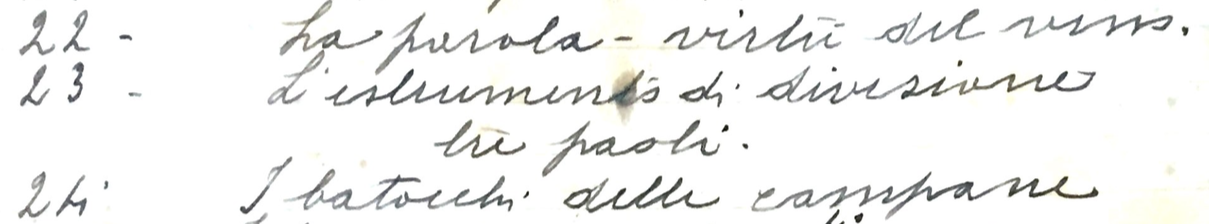
\includegraphics[width=\textwidth]{capitolo23}
    %\vspace{-0.3cm}
\end{figure}

 \begin{figure}[htb]
    \centering
    \vspace{-0.3cm}
    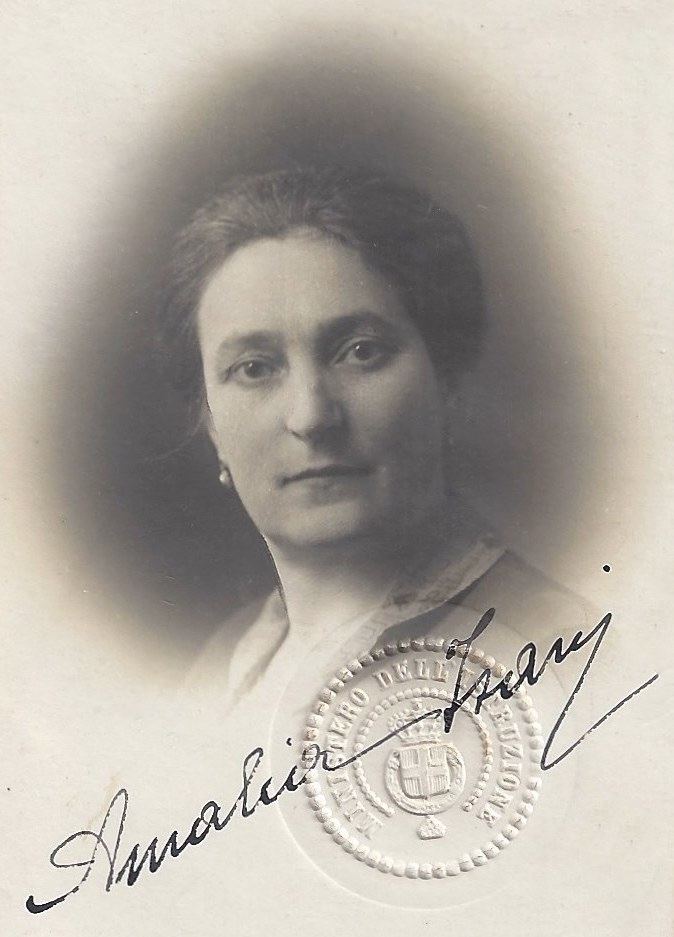
\includegraphics[width=\textwidth]{amalia}
    \caption[Amalia Isani]{\textbf{Amalia Isani}\index[Personaggi]{Isani Amalia}, moglie di Stefano Mingazzi\index[Personaggi]{Mingazzi Stefano}. Nacquero lo stesso giorno, il 3 agosto 1880. Fu maestra sia ad Alfonsine che a Ravenna.\label{fig:amalia}}
    \vspace{-0.7cm}
\end{figure}
